\begin{figure}[htbp]
\centering
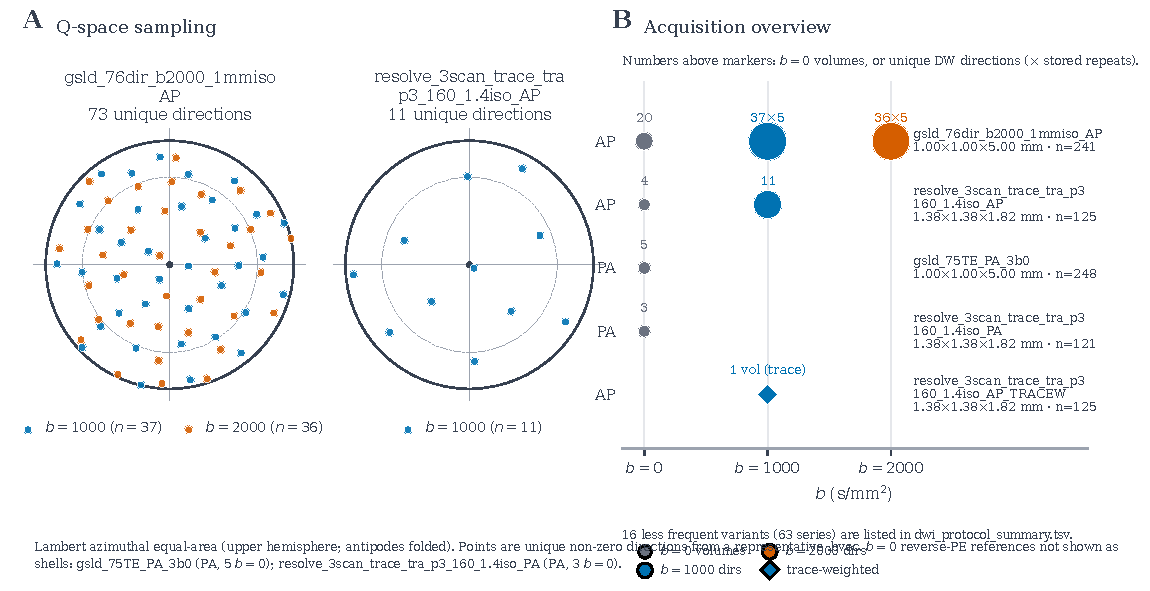
\includegraphics[width=\linewidth]{figures/Figure_DWI_protocols.pdf}
\caption{Diffusion MRI acquisition schemes in the released BIDS dataset. (A)~Angular distribution of unique non-zero diffusion-encoding directions from representative \texttt{.bvec} files, shown as a Lambert azimuthal equal-area projection of the upper hemisphere (antipodal directions folded). \texttt{gsld\_76dir\_b2000\_1mmiso\_AP} [AP: $b=1000$ ($n=37$ unique directions), $b=2000$ ($n=36$ unique directions)]; \texttt{resolve\_3scan\_trace\_tra\_p3\_160\_1.4iso\_AP} [AP: $b=1000$ ($n=11$ unique directions)]. Reverse-phase-encoding $b=0$ series (\texttt{gsld\_75TE\_PA\_3b0} [PA]; \texttt{resolve\_3scan\_trace\_tra\_p3\_160\_1.4iso\_PA} [PA]) are reference images and are not plotted as diffusion shells. (B)~Protocol-level summary of $b$-value shells, unique angular samples per shell, $b=0$ volume counts, voxel size, phase-encoding direction, and number of magnitude series for schemes represented in $\geq$20 series. The figure is derived from 923 released DWI NIfTI files in 131 sessions and shows unique acquisition schemes rather than every individual series. Where a gradient table stores repeated encodings of the same direction, panel~A plots unique directions and panel~B reports the observed repeat factor. 16 less frequent variants (truncated shells, alternate voxel size, missing phase-encoding metadata, or shim/PE differences) are tabulated in \texttt{dwi\_protocol\_summary.tsv}.}
\label{fig:dwi_protocols}
\end{figure}
